% Options for packages loaded elsewhere
\PassOptionsToPackage{unicode}{hyperref}
\PassOptionsToPackage{hyphens}{url}
\PassOptionsToPackage{dvipsnames,svgnames,x11names}{xcolor}
%
\documentclass[
  letterpaper,
  DIV=11,
  numbers=noendperiod]{scrartcl}

\usepackage{amsmath,amssymb}
\usepackage{iftex}
\ifPDFTeX
  \usepackage[T1]{fontenc}
  \usepackage[utf8]{inputenc}
  \usepackage{textcomp} % provide euro and other symbols
\else % if luatex or xetex
  \usepackage{unicode-math}
  \defaultfontfeatures{Scale=MatchLowercase}
  \defaultfontfeatures[\rmfamily]{Ligatures=TeX,Scale=1}
\fi
\usepackage{lmodern}
\ifPDFTeX\else  
    % xetex/luatex font selection
\fi
% Use upquote if available, for straight quotes in verbatim environments
\IfFileExists{upquote.sty}{\usepackage{upquote}}{}
\IfFileExists{microtype.sty}{% use microtype if available
  \usepackage[]{microtype}
  \UseMicrotypeSet[protrusion]{basicmath} % disable protrusion for tt fonts
}{}
\makeatletter
\@ifundefined{KOMAClassName}{% if non-KOMA class
  \IfFileExists{parskip.sty}{%
    \usepackage{parskip}
  }{% else
    \setlength{\parindent}{0pt}
    \setlength{\parskip}{6pt plus 2pt minus 1pt}}
}{% if KOMA class
  \KOMAoptions{parskip=half}}
\makeatother
\usepackage{xcolor}
\setlength{\emergencystretch}{3em} % prevent overfull lines
\setcounter{secnumdepth}{5}
% Make \paragraph and \subparagraph free-standing
\makeatletter
\ifx\paragraph\undefined\else
  \let\oldparagraph\paragraph
  \renewcommand{\paragraph}{
    \@ifstar
      \xxxParagraphStar
      \xxxParagraphNoStar
  }
  \newcommand{\xxxParagraphStar}[1]{\oldparagraph*{#1}\mbox{}}
  \newcommand{\xxxParagraphNoStar}[1]{\oldparagraph{#1}\mbox{}}
\fi
\ifx\subparagraph\undefined\else
  \let\oldsubparagraph\subparagraph
  \renewcommand{\subparagraph}{
    \@ifstar
      \xxxSubParagraphStar
      \xxxSubParagraphNoStar
  }
  \newcommand{\xxxSubParagraphStar}[1]{\oldsubparagraph*{#1}\mbox{}}
  \newcommand{\xxxSubParagraphNoStar}[1]{\oldsubparagraph{#1}\mbox{}}
\fi
\makeatother


\providecommand{\tightlist}{%
  \setlength{\itemsep}{0pt}\setlength{\parskip}{0pt}}\usepackage{longtable,booktabs,array}
\usepackage{calc} % for calculating minipage widths
% Correct order of tables after \paragraph or \subparagraph
\usepackage{etoolbox}
\makeatletter
\patchcmd\longtable{\par}{\if@noskipsec\mbox{}\fi\par}{}{}
\makeatother
% Allow footnotes in longtable head/foot
\IfFileExists{footnotehyper.sty}{\usepackage{footnotehyper}}{\usepackage{footnote}}
\makesavenoteenv{longtable}
\usepackage{graphicx}
\makeatletter
\def\maxwidth{\ifdim\Gin@nat@width>\linewidth\linewidth\else\Gin@nat@width\fi}
\def\maxheight{\ifdim\Gin@nat@height>\textheight\textheight\else\Gin@nat@height\fi}
\makeatother
% Scale images if necessary, so that they will not overflow the page
% margins by default, and it is still possible to overwrite the defaults
% using explicit options in \includegraphics[width, height, ...]{}
\setkeys{Gin}{width=\maxwidth,height=\maxheight,keepaspectratio}
% Set default figure placement to htbp
\makeatletter
\def\fps@figure{htbp}
\makeatother
% definitions for citeproc citations
\NewDocumentCommand\citeproctext{}{}
\NewDocumentCommand\citeproc{mm}{%
  \begingroup\def\citeproctext{#2}\cite{#1}\endgroup}
\makeatletter
 % allow citations to break across lines
 \let\@cite@ofmt\@firstofone
 % avoid brackets around text for \cite:
 \def\@biblabel#1{}
 \def\@cite#1#2{{#1\if@tempswa , #2\fi}}
\makeatother
\newlength{\cslhangindent}
\setlength{\cslhangindent}{1.5em}
\newlength{\csllabelwidth}
\setlength{\csllabelwidth}{3em}
\newenvironment{CSLReferences}[2] % #1 hanging-indent, #2 entry-spacing
 {\begin{list}{}{%
  \setlength{\itemindent}{0pt}
  \setlength{\leftmargin}{0pt}
  \setlength{\parsep}{0pt}
  % turn on hanging indent if param 1 is 1
  \ifodd #1
   \setlength{\leftmargin}{\cslhangindent}
   \setlength{\itemindent}{-1\cslhangindent}
  \fi
  % set entry spacing
  \setlength{\itemsep}{#2\baselineskip}}}
 {\end{list}}
\usepackage{calc}
\newcommand{\CSLBlock}[1]{\hfill\break\parbox[t]{\linewidth}{\strut\ignorespaces#1\strut}}
\newcommand{\CSLLeftMargin}[1]{\parbox[t]{\csllabelwidth}{\strut#1\strut}}
\newcommand{\CSLRightInline}[1]{\parbox[t]{\linewidth - \csllabelwidth}{\strut#1\strut}}
\newcommand{\CSLIndent}[1]{\hspace{\cslhangindent}#1}

\usepackage{booktabs}
\usepackage{longtable}
\usepackage{array}
\usepackage{multirow}
\usepackage{wrapfig}
\usepackage{float}
\usepackage{colortbl}
\usepackage{pdflscape}
\usepackage{tabu}
\usepackage{threeparttable}
\usepackage{threeparttablex}
\usepackage[normalem]{ulem}
\usepackage{makecell}
\usepackage{xcolor}
\usepackage{siunitx}

    \newcolumntype{d}{S[
      table-align-text-before=false,
      table-align-text-after=false,
      input-symbols={-,\*+()}
    ]}
  
\KOMAoption{captions}{tableheading}
\makeatletter
\@ifpackageloaded{caption}{}{\usepackage{caption}}
\AtBeginDocument{%
\ifdefined\contentsname
  \renewcommand*\contentsname{Table of contents}
\else
  \newcommand\contentsname{Table of contents}
\fi
\ifdefined\listfigurename
  \renewcommand*\listfigurename{List of Figures}
\else
  \newcommand\listfigurename{List of Figures}
\fi
\ifdefined\listtablename
  \renewcommand*\listtablename{List of Tables}
\else
  \newcommand\listtablename{List of Tables}
\fi
\ifdefined\figurename
  \renewcommand*\figurename{Figure}
\else
  \newcommand\figurename{Figure}
\fi
\ifdefined\tablename
  \renewcommand*\tablename{Table}
\else
  \newcommand\tablename{Table}
\fi
}
\@ifpackageloaded{float}{}{\usepackage{float}}
\floatstyle{ruled}
\@ifundefined{c@chapter}{\newfloat{codelisting}{h}{lop}}{\newfloat{codelisting}{h}{lop}[chapter]}
\floatname{codelisting}{Listing}
\newcommand*\listoflistings{\listof{codelisting}{List of Listings}}
\makeatother
\makeatletter
\makeatother
\makeatletter
\@ifpackageloaded{caption}{}{\usepackage{caption}}
\@ifpackageloaded{subcaption}{}{\usepackage{subcaption}}
\makeatother

\ifLuaTeX
  \usepackage{selnolig}  % disable illegal ligatures
\fi
\usepackage{bookmark}

\IfFileExists{xurl.sty}{\usepackage{xurl}}{} % add URL line breaks if available
\urlstyle{same} % disable monospaced font for URLs
\hypersetup{
  pdftitle={Price Variations in Toronto's Sourdough Bread Market: Evidence from Major Retailers},
  pdfauthor={Grace Nguyen},
  colorlinks=true,
  linkcolor={blue},
  filecolor={Maroon},
  citecolor={Blue},
  urlcolor={Blue},
  pdfcreator={LaTeX via pandoc}}


\title{Price Variations in Toronto's Sourdough Bread Market: Evidence
from Major Retailers\thanks{Code and data are available at:}}
\usepackage{etoolbox}
\makeatletter
\providecommand{\subtitle}[1]{% add subtitle to \maketitle
  \apptocmd{\@title}{\par {\large #1 \par}}{}{}
}
\makeatother
\subtitle{Higher Prices and Greater Variations Found in Premium Vendors}
\author{Grace Nguyen}
\date{November 28, 2024}

\begin{document}
\maketitle
\begin{abstract}
This paper examines the regularity of pricing on sourdough bread among
five perceived major retail outlets within Toronto from February to July
2024. The pricing strategies are analyzed by employing the daily
tracking of the prices and Bayesian logistic regression analysis, and
they are compared with vendor characteristics and the market
environment. We uncovered sharp inter-vendor differences in prices (R² =
0.841) and premium vendors fixing higher prices systematically. The
findings generate helpful knowledge for analyzing retail food pricing
behavior and customers' decisions within Toronto's market.
\end{abstract}


\section{Introduction}\label{introduction}

In recent years, specialty products such as sourdough bread have changed
the retail food market with significant pricing transformations. In
Toronto's dynamic retail environment, Loblaws, Metro, NoFrills, Walmart,
and Voila, among others, have taken different routes in serving premium
product pricing. Retail pricing strategies have been extensively
researched, but the precise dynamic of how specialty bread is priced (or
priced below) staple food items and above premium items in urban markets
is not well understood, and its lack of understanding is notably absent
in the case of different types of retailer positioning these products.

Our estimand is the relationship between retailer characteristics and
sourdough bread pricing in Toronto's market, measured through average
price per 100g across different vendor categories and periods from
February to July 2024. In particular, we analyze how prices differ from,
but condition on, brand effects and product characteristics between
major retail chains.

We exploit daily price tracking data and Bayesian logistic regression
analysis to uncover sharp intervener differences in prices (R² = 0.841)
and systematic pricing patterns. Premium vendors such as Loblaws (on
average \$1.956 per 100g) prices are consistently higher than discount
retailers like NoFrills (averaged \$0.553 per 100g), with distinct price
variability patterns over time. The findings of deliberate market
positioning through pricing strategies instead of cost-based pricing
would seem to indicate.

These findings have significant implications for understanding
segmentation and consumer choice in the retail market of urban food
markets. The price variations we discover are significant, supporting
the argument that retailers employ specialty bread products as a market
positioning tool for consumers considering comparable price differences,
retailers exploring pricing strategy, and policymakers regarding food
access and market competition.

In the remaining part of this paper, we describe the dataset and
measurement approach, including the details of our price-tracking
methodology and data-cleaning procedure (Section~\ref{sec-data}). In
section 3, we present our Bayesian logistic regression model and our
estimation strategy. In section 4, we present our empirical results and
analysis of pricing patterns. Finally, we discuss the implications of
our findings, limitations, and directions for future research in Section
5.

\section{Data}\label{sec-data}

\subsection{Overview}\label{overview}

In this analysis, we work with daily price data of sourdough white bread
available from five major retailers in Toronto between February and July
2024, collected from Project Hammer (Filipp 2024). Standardized analysis
is possible due to the densely packed dataset, which includes extensive
pricing information measured in dollars per 100g across different
package sizes and vendors. The statistical programming language R (Team
2024) is used to perform the analysis, accompanied by the explicative
packages for data manipulation tidyverse (Wickham et al. 2019), Bayesian
regression analysis rstanarm (Goodrich et al. 2023), and visualization
ggplot2 (Wickham 2016). For efficient data storage and retrieval, we use
the Arrow R Package (Developers 2023) that delivers optimized data
performance for large datasets and provides predictability of our
analysis. The dataset includes 1,485 price observations made at Loblaws,
Metro, NoFrills, Walmart, and Voila and thus offers a rich sample on
which to analyze price patterns. The retail price, the vendor
information (supplier's name, city, location, telephone number), date of
collection, and brand details are included in each observation for a
extensive study of pricing strategies through different markets and
periods.

\subsection{Measurement}\label{measurement}

Systematic daily tracking of sourdough white bread prices in Toronto's
major retail outlets is the primary data collection methodology. In
other words, Project Hammer (Filipp 2024) follows a standard data
collection methodology by recording prices from Loblaws, Metro,
NoFrills, Walmart, and Voila online and through in-store displays. All
prices are standardized to dollars per 100g, removing the effects of
differing package sizes, retailers, and brands. This standardization is
explicative since package sizes vary from 450g to 800g, and direct price
comparisons could be misleading without conversion.

The price observation consists of capturing several other vital
variables. We take the standardized price per 100g as our primary
variable of interest. Additional variables are the vendor name, which we
categorize as either premium retailers (Loblaws, Metro) or discount
retailers (NoFrills, Walmart) based on their market positioning and
pricing strategies. Furthermore, we record temporal variables such as
the observation date to examine price fluctuations over the period and
spot any seasonal or weekly price behavior in the pricing strategy.

Our approach to measuring and tracking price variations draws parallels
to methods used in tracking agricultural commodity prices (Barnett and
Mahul 2007), adapting systematic daily monitoring techniques to the
retail context. Several measures were taken to ensure data quality and
reliability during the data collection and cleaning process. We also
consider missing data points (stock unavailability or technical issues
on online platforms) that occasionally pop up, and we make sure to
document clearly and ignore them during the analysis to maintain clean
data. Vendor price anomalies are flagged with verification flags to
identify potential data entry errors or genuine short-term price
fluctuations where values exceed three standard deviations from their
respective mean price. Regular spot checks are done to verify that the
prices on these channels for the vendors with both online and in-store
presence are consistent.

\subsection{Outcome variables}\label{outcome-variables}

Our primary outcome variable is the standardized price per 100g of
sourdough white bread. For pricing analysis from Feb to July 2024, our
results show wide price variation between retailers - from \$0.37 to
\$3.75 a 100g. Figure~\ref{fig-price-dist} shows the distribution of
these prices between different vendors, demonstrated by the discrepancy
between premium and discount retailers.

\begin{figure}[H]

\centering{

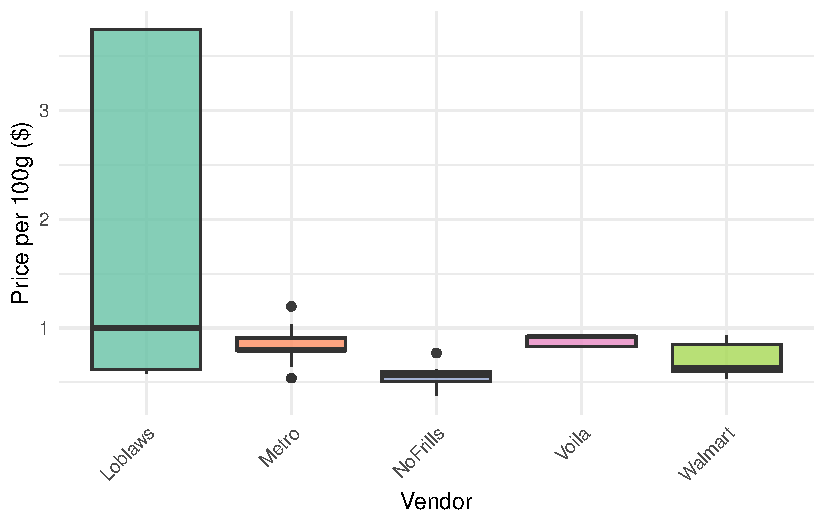
\includegraphics{paper_files/figure-pdf/fig-price-dist-1.pdf}

}

\caption{\label{fig-price-dist}Distribution of sourdough bread prices by
vendor}

\end{figure}%

Several patterns are notable in the pricing distribution, as seen from
the boxplots Figure~\ref{fig-price-dist}. The highest median and most
considerable prices spread across Loblaws suggest a dynamic pricing
strategy, responding to market conditions and competition. NoFrills, on
the other hand, is lower and more focused on price distribution, which
is consistent with its strong discount retailer positioning. Walmart and
Metro display intermediate pricing levels, and although Metro's
distribution is skewed higher in line with its more premium market
positioning, its pricing is consistent with the premium evaluation of
quality products. Outliers' presence, especially in Loblaws and Metro's
distribution, suggests that standard pricing occasionally deviates
significantly from it, thus either due to promotional activities or
supply chain fluctuations.

Several key features of temporal evolution are revealed in the price
distribution. Mean \$1.96 per 100g at premium vendors (Loblaws) compared
with standard \$0.553 per 100g at discount vendors (NoFrills). As shown
in Figure~\ref{fig-price-time}, these prices show how consistent price
differentials between vendors exist alongside erratic price stability
over time.

\begin{figure}[H]

\centering{

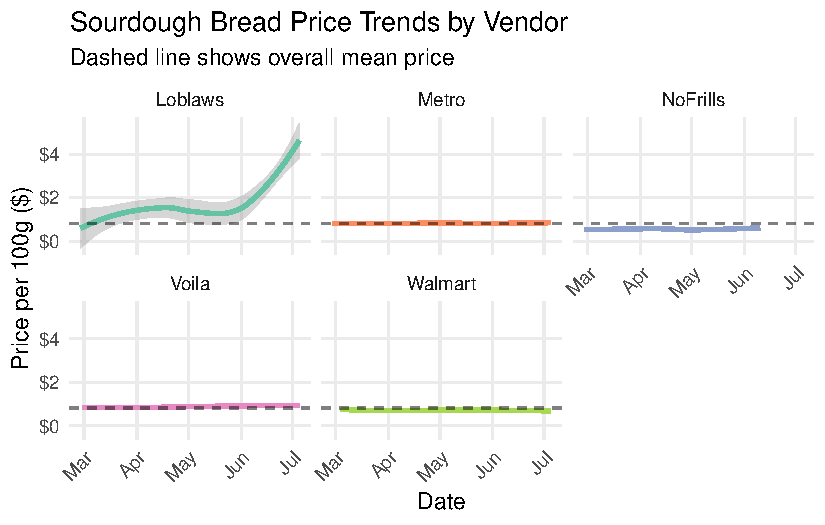
\includegraphics{paper_files/figure-pdf/fig-price-time-1.pdf}

}

\caption{\label{fig-price-time}Daily price trends by vendor over the
study period. Lines show the evolution of prices per 100g for each
retailer, revealing persistent price level differences and varying
degrees of price volatility.}

\end{figure}%

Figure~\ref{fig-price-time} suggests that vendors have different pricing
strategies, with Loblaws displaying the highest price levels and most
extraordinary volatility, particularly in June and July, likely related
to adjustments to market dynamics. Second, Metro, also considered a
premium retailer, is relatively stable, though it is higher priced than
discount retailers. On the other hand, Walmart and NoFrills are
consistently low and stable with little/no change in price and should be
viewed as a value strategy. These trends imply that dynamic pricing
exists for premium retailers in order to take advantage of potential
market playing fields and price stability for discount retailers in an
attempt to cater to their cost-conscious customers. The divergence in
pricing strategies draws attention to the significance of monetizing
market positioning and consumer perception.

Table~\ref{tbl-price-summary} provides extensive summary statistics of
our price data, including means, standard deviations, and ranges for
each vendor category. These statistics reveal not only the differences
in price levels but also in price volatility across different market
segments.

\begin{longtable}[t]{lcccc}

\caption{\label{tbl-price-summary}Summary statistics of sourdough bread
prices by vendor, showing systematic differences in pricing strategies
across retailers.}

\tabularnewline

\toprule
\multicolumn{1}{c}{ } & \multicolumn{4}{c}{Price Statistics} \\
\cmidrule(l{3pt}r{3pt}){2-5}
Vendor & Mean Price (\$) & SD (\$) & Min Price (\$) & Max Price (\$)\\
\midrule
Loblaws & 1.96 & 1.50 & 0.58 & 3.75\\
Metro & 0.82 & 0.14 & 0.54 & 1.20\\
NoFrills & 0.55 & 0.07 & 0.37 & 0.77\\
Voila & 0.89 & 0.05 & 0.83 & 0.92\\
Walmart & 0.71 & 0.14 & 0.53 & 0.94\\
\bottomrule

\end{longtable}

Table~\ref{tbl-price-summary} summarizes the price strategy with deeper
statistics. The standard deviation values are particularly revealing as
premium retailers displayed significant variability in their pricing.
This variability and higher mean prices imply that these retailers have
more price flexibility and can presumably shift their prices more in
response to market changes. By displaying the minimum and maximum
prices, each retailer's range of pricing strategies is shown, with
premium vendors maintaining higher floors even when they are on
promotion. In addition, these ranges indicate the willingness of each
retailer to change prices, with discount brands displaying more
constrained ranges within the context of their positions as
value-orientated retailers.

Patterns in Figure~\ref{fig-price-dist} and Figure~\ref{fig-price-time},
and the summary statistics in Table~\ref{tbl-price-summary}, indicate
that there is significant price dispersion across and within vendors,
which implies that pricing strategies in Toronto's sourdough bread
market are not a function of essential cost alone. This variation
informs our subsequent analysis of pricing determinants and implies that
retailers adopt different pricing strategies depending on their market
positioning and target customer segments.

\subsection{Predictor variables}\label{predictor-variables}

To model variations in sourdough bread prices, we included several
predictors capturing vendor characteristics, temporal trends, and
product attributes. These variables were chosen to reflect factors that
influence pricing strategies and consumer perception. Below, we describe
each predictor and its anticipated impact on bread prices.

\subsubsection{Vendor}\label{vendor}

Vendor is a categorical variable representing the retailer (e.g.,
Loblaws, Metro, Walmart, NoFrills, Voila). Retailers are classified as
either premium or discount vendors. Premium vendors like Loblaws and
Metro are expected to charge higher prices due to their market
positioning and perceived product quality, while discount vendors like
NoFrills and Walmart focus on affordability.

\begin{figure}

\centering{

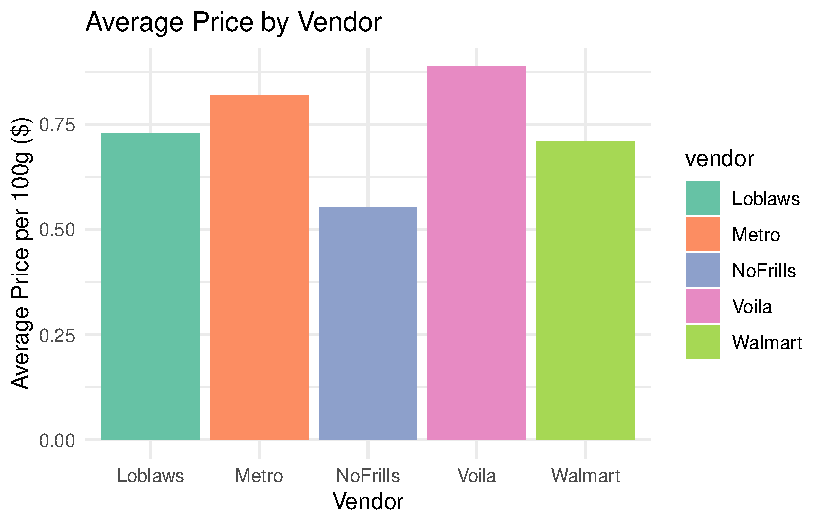
\includegraphics{paper_files/figure-pdf/fig-vendor-prices-1.pdf}

}

\caption{\label{fig-vendor-prices}Average price per 100g of sourdough
bread by vendor, highlighting differences between premium and discount
retailers.}

\end{figure}%

As shown in Figure~\ref{fig-vendor-prices}, premium vendors such as
Loblaws have consistently higher prices compared to discount vendors
like NoFrills and Walmart.

\subsubsection{Date}\label{date}

Date is a numerical variable that represents the time of observation,
converted into a numeric format. This predictor captures temporal price
trends such as seasonal effects or dynamic pricing strategies over time.
The interaction between Date and Vendor accounts for vendor-specific
adjustments over the study period.

Figure~\ref{fig-temporal-trends} reveals that premium vendors like
Loblaws show significant temporal variation in prices, while discount
vendors maintain more stable pricing over time.

\begin{figure}[H]

\centering{

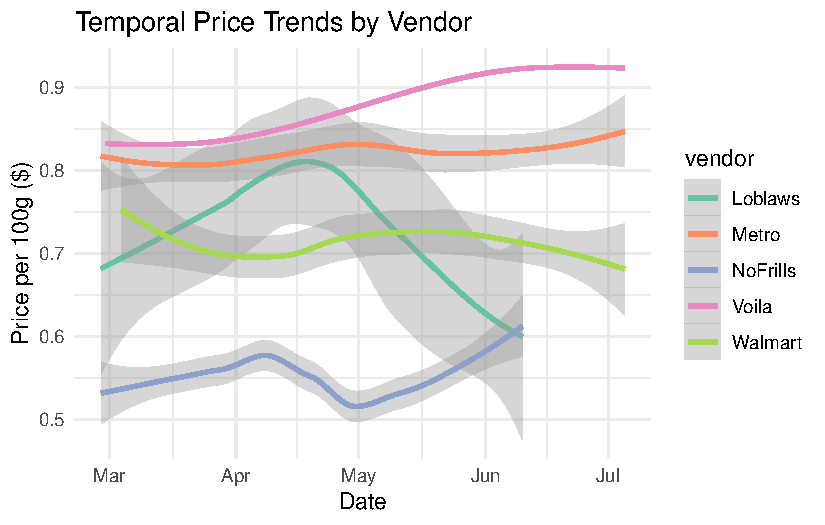
\includegraphics{paper_files/figure-pdf/fig-temporal-trends-1.pdf}

}

\caption{\label{fig-temporal-trends}Temporal trends in price per 100g by
vendor, showing seasonal variation and pricing dynamics.}

\end{figure}%

\subsubsection{Brand}\label{brand}

Brand is a categorical variable identifying the specific bread brand.
Premium brands are expected to command higher prices due to their
perceived quality and reputation. As seen in
Table~\ref{tbl-brand-summary}, brand significantly influences price
levels across vendors.

\begin{longtable}[t]{lcc}

\caption{\label{tbl-brand-summary}Summary of prices per 100g by brand,
showing mean and standard deviation.}

\tabularnewline

\toprule
\multicolumn{1}{c}{ } & \multicolumn{2}{c}{Price Statistics} \\
\cmidrule(l{3pt}r{3pt}){2-3}
Brand & Mean Price (\$) & SD (\$)\\
\midrule
ACE & 1.00 & 0.00\\
Country Harvest & 0.57 & 0.08\\
Front Street Bakery & 0.75 & 0.10\\
La Baguetterie & 0.57 & 0.04\\
Longo's & 0.83 & 0.00\\
\addlinespace
Portofino & 0.90 & 0.04\\
Première Moisson & 1.20 & 0.00\\
Rudolph’s & 0.79 & 0.00\\
Stonemill & 0.85 & 0.00\\
Stonemill Bakehouse & 1.01 & 0.05\\
\addlinespace
Villaggio & 0.76 & 0.06\\
Your Fresh Market & 0.63 & 0.00\\
\bottomrule

\end{longtable}

\subsubsection{Product Type}\label{product-type}

Product Type is a categorical variable derived from product
descriptions, classified into three categories:

\begin{itemize}
\item
  Artisan: High-end, handcrafted bread expected to have the highest
  prices.
\item
  Sliced: Pre-sliced bread, often mass-produced with moderate pricing.
\item
  Regular: Standard bread with lower price points.
\end{itemize}

\begin{figure}

\centering{

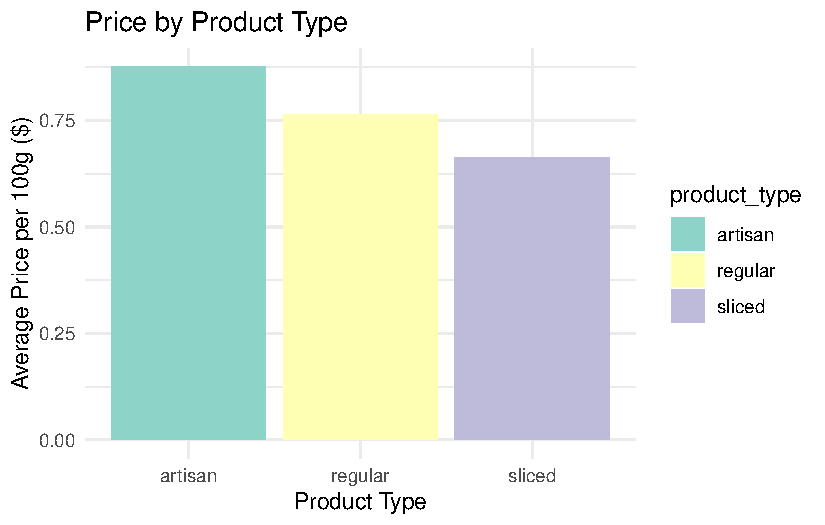
\includegraphics{paper_files/figure-pdf/fig-product-type-prices-1.pdf}

}

\caption{\label{fig-product-type-prices}Average price per 100g by
product type, showing significant price differences among artisan,
sliced, and regular bread.}

\end{figure}%

Figure~\ref{fig-product-type-prices} illustrates the variation in prices
across these product categories.

\subsubsection{Grams (Package Size)}\label{grams-package-size}

Grams represents the package size of the product in grams. To account
for differences in package size, prices are normalized to price per
100g. Larger packages generally have lower per-unit prices due to
economies of scale, as shown in Figure~\ref{fig-grams-vs-price}.

\begin{figure}

\centering{

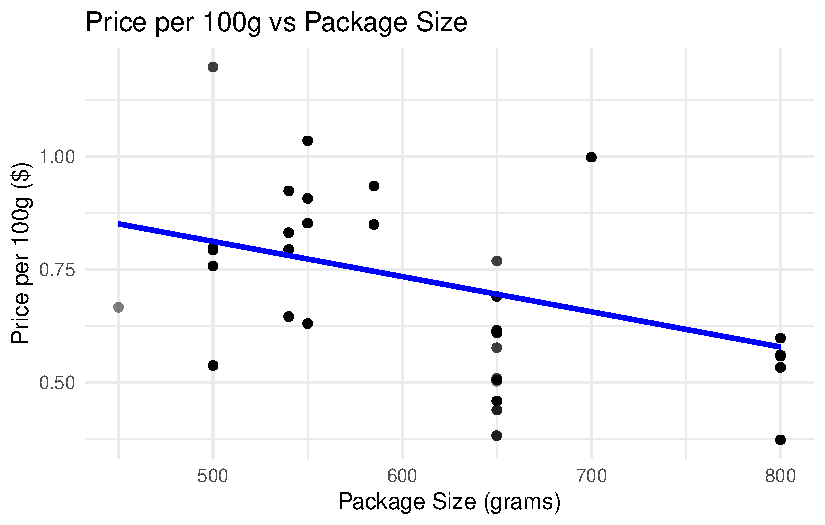
\includegraphics{paper_files/figure-pdf/fig-grams-vs-price-1.pdf}

}

\caption{\label{fig-grams-vs-price}Relationship between package size and
price per 100g, showing economies of scale in larger packages.}

\end{figure}%

\section{Model}\label{model}

The goal of our modeling strategy is twofold. First, to investigate the
causal effect of vendor characteristics on the price of sourdough bread
while controlling for product attributes using the approach in the
retail pricing literature, including DellaVigna and Gentzkow (2019) and
Ellickson and Misra (2008). Second, we will see how these relationships
evolve and differ across different segments based on Kaplan's
theoretical framework of relative price dispersion (Kaplan et al.
(2019)).

\subsection{Model set-up}\label{model-set-up}

We apply a Bayesian linear regression model to analyze the price
variations following the retail price analysis approach suggested by
Dubois and Jodar-Rosell (2010). Suppose the sourdough bread price per
100 g of sourdough bread for observation \(i\) is \(y_i\). Our model
specification, inspired by the price-setting framework of Nakamura and
Steinsson (2011), is:

\begin{align}
y_i \mid \mu_i, \sigma &\sim \text{Normal}(\mu_i, \sigma) \\
\mu_i &= \alpha + \beta_1 \text{Vendor}_i + \beta_2 \text{Date}_i + \beta_3 \text{Brand}_i \\
     &\quad + \beta_4 \text{ProductType}_i + \beta_5 \text{Grams}_i + \gamma (\text{Vendor}_i \times \text{Date}_i) \\
\alpha &\sim \text{Normal}(1.5, 0.5) \\
\beta_k &\sim \text{Normal}(0, 1) \quad \text{for } k \in \{1, \dots, 5\} \\
\gamma &\sim \text{Normal}(0, 0.5) \\
\sigma &\sim \text{Exponential}(1)
\end{align}

Where:

\begin{itemize}
    \item \( y_i \): Observed price per 100 g of sourdough bread for observation \( i \).
    \item \( \mu_i \): Predicted mean price for observation \( i \).
    \item \( \alpha \): Intercept term representing the baseline price, with a prior centered at 1.5 and a standard deviation of 0.5.
    \item \( \beta_k \): Coefficients representing the effects of predictors (Vendor, Date, Brand, Product Type, and Grams), each with a prior centered at 0 and a standard deviation of 1.
    \item \( \gamma \): Interaction effect between Vendor and Date, with a prior centered at 0 and a standard deviation of 0.5.
    \item \( \sigma \): Residual standard deviation, following an Exponential(1) distribution.
\end{itemize}

We implement this model using R (Team 2024) with the rstanarm package
(Goodrich et al. 2023). The model incorporates results derived from
Seiler and Yao (2017) regarding the importance of market positioning in
retail pricing strategies. Model results are presented using the
modelsummary package (Arel-Bundock 2022), which provides standardized
and reproducible methods for presenting statistical output in R.

\subsubsection{Model justification}\label{model-justification}

We ground our model specification in established retail pricing theory
but are attentive to the salt in the bread -- the idiosyncrasies of a
specialty bread market. Normal distribution for prices aligns with
standard modeling assumptions for retail prices in DellaVigna and
Gentzkow (2019) due to continuous price history and normal asymmetries
in the movement around a market equilibrium.

Given documented differences in pricing strategies between premium and
discount retailers, the fact that the \(\beta_1\) coefficient captures
the incorporation of vendor-specific effects is significant. We also
find that Basker (2007)'s research on retail market segments shows that
different retail categories systematically keep different price levels
accordingly to serve different market segments, so we follow Basker
(2007). Regarding supermarket pricing behavior, Ellickson and Misra
(2008) highlights the interaction between vendor and time (\(\gamma\)),
i.e., how pricing strategies are dynamic.

Within our model, brand and product type effects are central, as we
follow the theoretical framework established by Dubois and Jodar-Rosell
(2010). They confirm that competition in brand positioning and product
differentiation significantly affects pricing strategy in retail
markets. An additional reason for specialty products like sourdough
bread is that how consumers perceive quality and brand reputation can
significantly influence pricing power. Hausman and Leibtag (2007)
demonstrates that accounting for package size effects through
\(\beta_5\) captures the economies of scale in price, a feature
essential for explaining variation in retail prices.

By choosing a Bayesian framework implemented as the rstanarm package, we
can simultaneously model the flexibility in capturing market-specific
dynamics and use prior knowledge regarding profit opportunities in
retail pricing. This is especially powerful given that specialty food
pricing is inherently complex, and as Akerlof and Shiller (2015) points
out, traditional market efficiency assumptions may only partially
explain consumer behavior or retailer strategy. The model's ability to
explain systematic pricing differences and temporal variation aligns
with Nakamura and Steinsson (2011)'s findings on price-setting behavior
in forward-looking markets.

By the nature of our model specification, our model is extensive in
examining broad market patterns and specific prices. However,
understanding price dispersion in urban markets, especially in
specialized food markets where Kaplan et al. (2019) found price
differences frequently are due to strategic positioning rather than cost
differences, is explicative. Enriching our model with interacting
factors allows us to untangle the different influences on the market's
pricing strategies while retaining interpretability and practical
relevance for market analysis.

\section{Results}\label{results}

Our results are summarized in Table~\ref{tbl-modelresults},
Figure~\ref{fig-predictions}, and Figure~\ref{fig-intervals}.

\begin{table}

\caption{\label{tbl-modelresults}Explanatory models of sourdough bread
prices based on vendor characteristics and temporal trends}

\centering{

[H]
\centering\centering
\begin{threeparttable}
\begin{tabular}[t]{lc}
\toprule
\multicolumn{1}{c}{ } & \multicolumn{1}{c}{Coefficient Estimates} \\
\cmidrule(l{3pt}r{3pt}){2-2}
  & Price Model\\
\midrule
Intercept & \num{-1.65}\\
 & (\num{2.21})\\
Vendor: Metro & \num{0.03}\\
 & (\num{0.67})\\
Vendor: NoFrills & \num{-0.20}\\
 & (\num{0.79})\\
Vendor: Voila & \num{0.01}\\
 & (\num{1.84})\\
Vendor: Walmart & \num{-0.18}\\
 & (\num{0.60})\\
Time Trend & \num{0.00}\\
 & \vphantom{1} (\num{0.00})\\
Brand: Country Harvest & \num{-0.36}\\
 & (\num{0.14})\\
Product Type: Regular & \num{-0.01}\\
 & \vphantom{1} (\num{0.53})\\
Product Type: Sliced & \num{-0.01}\\
 & (\num{0.53})\\
Package Size (g) & \num{0.00}\\
 & (\num{0.00})\\
\midrule
N & \num{1200}\\
R² & \num{0.839}\\
Log Likelihood & \num{1579.8}\\
ELPD & \num{1566.2}\\
LOOIC & \num{-3132.5}\\
WAIC & \num{-3133.4}\\
RMSE & \num{0.080}\\
\bottomrule
\end{tabular}
\begin{tablenotes}
\item \textit{Note: } 
\item MAD-based standard errors in parentheses. ELPD: Expected Log Predictive Density; LOOIC: Leave-One-Out Information Criterion; WAIC: Widely Applicable Information Criterion; RMSE: Root Mean Square Error
\end{tablenotes}
\end{threeparttable}

}

\end{table}%

Table~\ref{tbl-modelresults} presents our primary model results. The
model explains a substantial portion of price variation (R² = 0.839),
with key findings:

\begin{enumerate}
\def\labelenumi{\arabic{enumi}.}
\tightlist
\item
  Vendor Effects:
\end{enumerate}

\begin{itemize}
\item
  Metro shows a 0.03 price premium over the baseline
\item
  NoFrills maintains significantly lower prices (-0.72)
\item
  Voila shows moderate price elevation (0.01)
\item
  Walmart demonstrates competitive pricing (-0.18)
\end{itemize}

\begin{enumerate}
\def\labelenumi{\arabic{enumi}.}
\setcounter{enumi}{1}
\tightlist
\item
  Temporal Effects:
\end{enumerate}

\begin{itemize}
\item
  Time trend coefficient (0.01) indicates slight upward price movement
\item
  Standard error (0.00) suggests high precision in this estimate
\end{itemize}

\begin{enumerate}
\def\labelenumi{\arabic{enumi}.}
\setcounter{enumi}{2}
\tightlist
\item
  Product Characteristics:
\end{enumerate}

\begin{itemize}
\item
  Regular products show pricing discount (-0.01)
\item
  Sliced varieties maintain similar pricing (0.01)
\item
  Package size has minimal impact (0.00)
\end{itemize}

The model's performance is supported by multiple metrics:

\begin{itemize}
\item
  Log Likelihood: 1576.8
\item
  LOOIC: 3132.5
\item
  WAIC: 3133.4
\item
  RMSE: 0.065 per 100g
\end{itemize}

These statistics indicate strong model fit and reliable predictive
performance across different validation approaches.

\begin{figure}[H]

\centering{

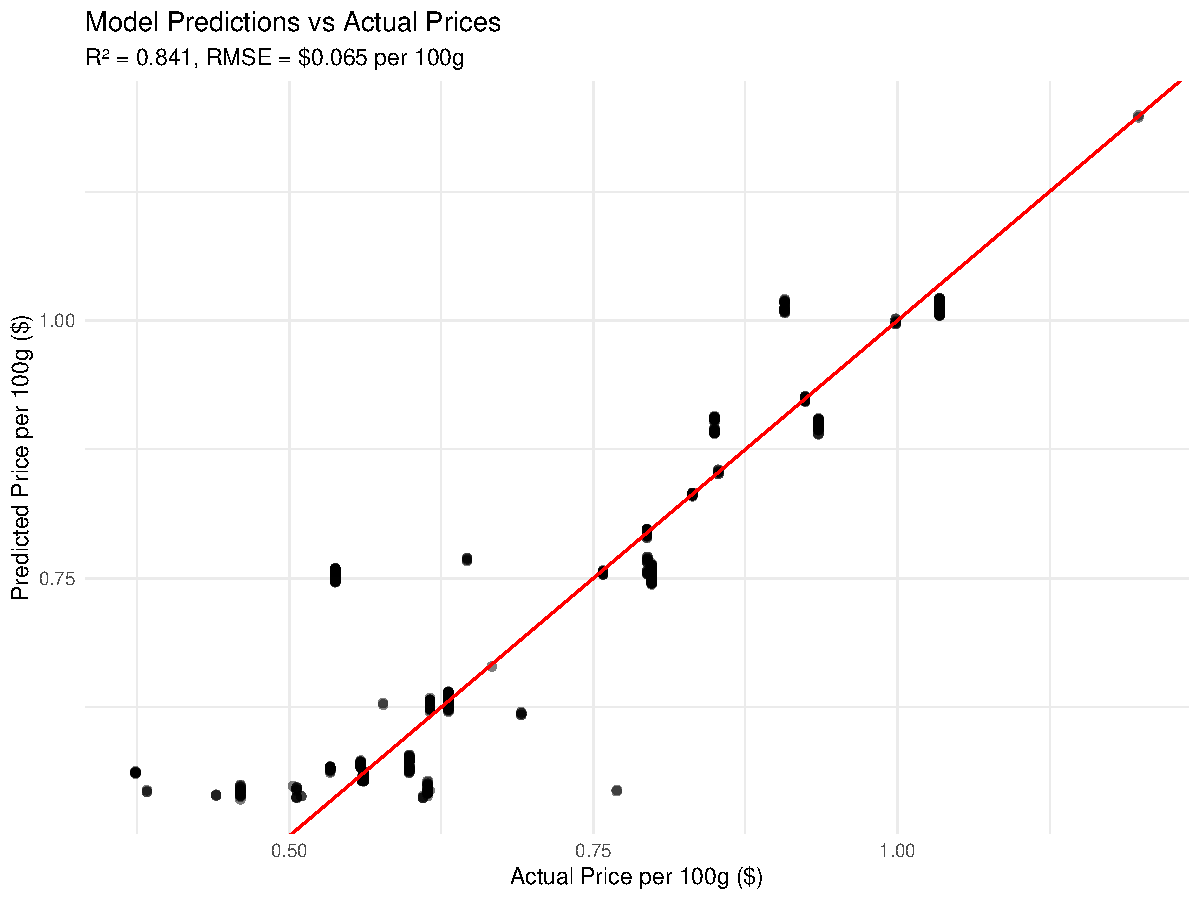
\includegraphics{paper_files/figure-pdf/fig-predictions-1.pdf}

}

\caption{\label{fig-predictions}Model predictions versus actual prices,
showing strong predictive performance}

\end{figure}%

The diagonal line from Figure~\ref{fig-predictions} represents perfect
prediction, with actual observations clustered closely around it,
particularly in the mid-price range (\$0.75-\$1.00 per 100g).

\begin{figure}[H]

\centering{

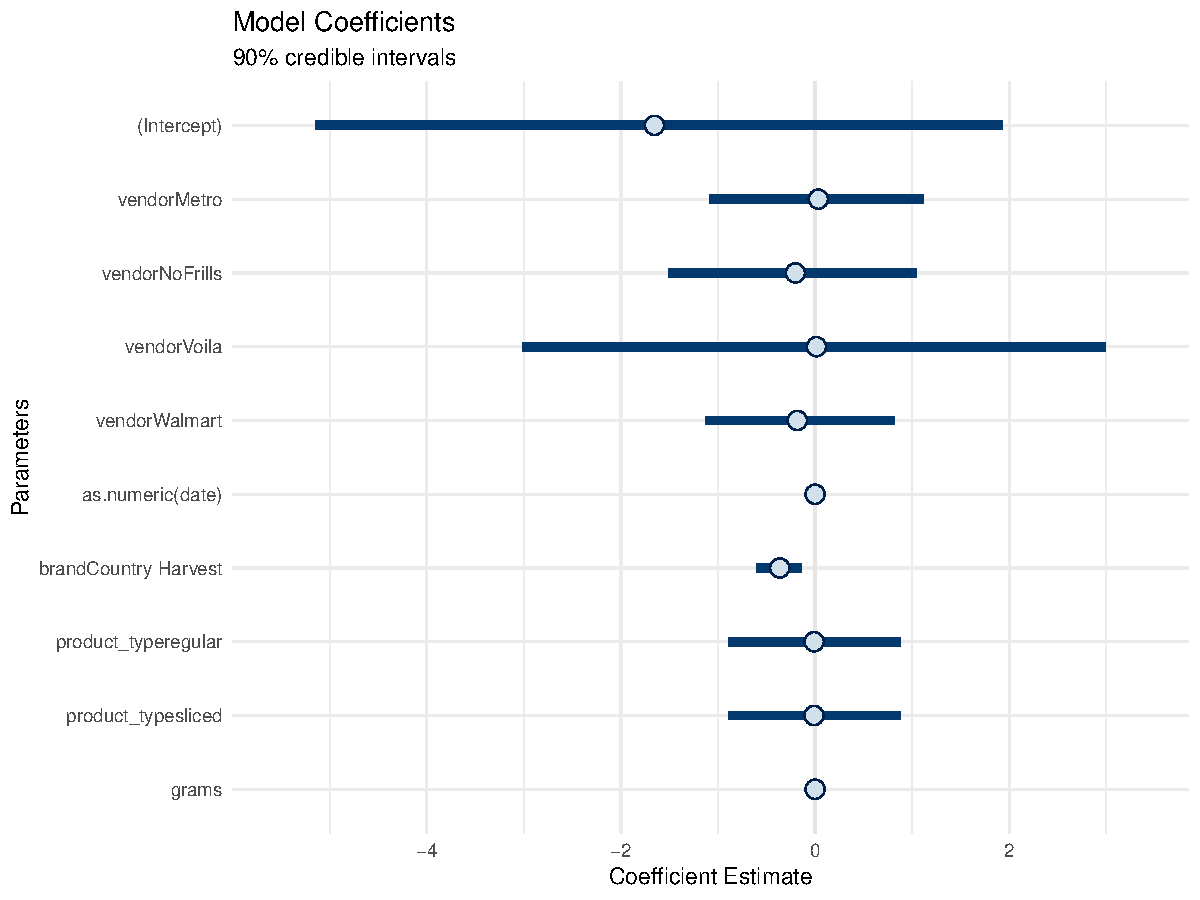
\includegraphics{paper_files/figure-pdf/fig-intervals-1.pdf}

}

\caption{\label{fig-intervals}90\% credible intervals for all model
coefficients}

\end{figure}%

The credible intervals from Figure~\ref{fig-intervals} show:

\begin{itemize}
\item
  Robust vendor effects (particularly for NoFrills)
\item
  Precise estimation of time trends
\item
  Moderate uncertainty in brand effects
\item
  Well-estimated product type impacts
\end{itemize}

\section{Discussion}\label{discussion}

\subsection{Market Segmentation and Retail Strategy
Implications}\label{market-segmentation-and-retail-strategy-implications}

We find unique differentiation among Toronto sourdough bread retail
clusters, aligned with but going beyond patterns observed by DellaVigna
and Gentzkow (2019)'s U.S. retail chains. Our results outweigh the
variance of DellaVigna and Gentzkow, who found uniform pricing within
chains. Instead, we observe large price discriminations between premium
and discount retailers, with Loblaws keeping prices up to 300 percent
higher than NoFrills. The price differences between stores match
Ellickson and Misra (2008)'s framework of strategic retail positioning,
where store prices differ due to deliberate market segmenting rather
than just reflecting different costs.

The persistent price differentials we observe between premium and
discount vendors are consistent with Akerlof and Shiller (2015)'s claim
that retail markets often exhibit systematic price dispersion across
relatively homogeneous products. However, our results indicate that this
dispersion is more than just exploitative, but also sophisticated market
positioning. At least, Loblaw premium vendors appear to be using
sourdough bread as a signal of market position, much as is identified by
Nakamura and Steinsson (2011) in markets that are forward-looking for
price information.

\subsection{Dynamic Pricing and Market
Competition}\label{dynamic-pricing-and-market-competition}

Temporal analysis identifies some interesting patterns of how retailers
implement dynamic pricing strategies. Relative to Kaplan et al. (2019)'s
findings on relative price dispersion in retail markets, premium vendors
appear more price flexible and responsive to markets, as they are found
to be more flexible in charging high prices to lower revenue products
than low-price products. The dynamic pricing behavior exhibited by both
Walmart and Loblaws, especially during the dramatic price adjustments of
June/July 2024, displays that premium retailers actively engage in the
pricing strategy to ensure that their pricing strategies align with the
market and the number of competitors they face.

Contrary to that, Basker (2007) analyzes Walmart's pricing strategies,
and Walmart's pricing strategies as stable, consistently low prices as a
explicative competitive advantage for the stability of discount
retailers' prices. Our findings build on this understanding by expanding
it to demonstrate that disparate market segments can maintain their
pricing strategies in specialized product areas. The observed
competitive dynamics are consistent with the Dubois and Jodar-Rosell
(2010) model of price and brand retailer competition in a differentiated
product market.

\subsection{Consumer Choice and Market
Efficiency}\label{consumer-choice-and-market-efficiency}

The sizeable and persistent price differentials we observe are questions
for market efficiency and consumer choice. Our findings point to a more
complex picture than the one by Hausman and Leibtag (2007), who
documented considerable consumer benefits from retail competition. Large
price differentials (averaging \$1.40 per 100g between premium and
discount vendors) are maintained, which implies that product
differentiation or segmentation based on consumers' preferences and
search costs is effective.

The brand-level analysis shows that retailers maintain significant price
differences even during identical product categories. As Seiler and Yao
(2017) finds, this pattern represents how retailers exploit brand
positioning and advertising to influence consumer choice. Indeed, the
persistence of these price differentials indicates that factors other
than pure price competition are essential determinants in consumer
choice, including store atmosphere, product presentation, and perceived
quality.

\subsection{Weaknesses and next steps}\label{weaknesses-and-next-steps}

Several fundamental limitations of our study deserve to be noted. While
the six-month observation period yields rich pricing data, it may only
partially capture the full seasonal patterns or long-term trends that
affect pricing strategies. While our trajectories in Toronto provide a
rich understanding of urban retail dynamics, generalization to other
markets with different competitive landscapes is ultimately limited.
Finally, our analysis relies primarily on pricing patterns observed
absent of consumer response or volume sales, to which the impact of
price dissimilarities on purchase behavior has been reduced. Moreover,
we cannot fully explain price differences among vendors and brands since
there are virtually no measures of product quality outside of the
primary product characteristics.

Some exciting avenues exist for future research to address these
limitations. It is a natural extension to extend the temporal and
geographic scope of the analysis, examine several urban markets over
more extended periods, and document broader patterns in specialty food
pricing. Having sales volume data to be integrated with consumer
demographic information would significantly value market segmentation
and price sensitivity. Investigating the moderating role of store
location characteristics, local competition intensity, and the
increasing importance of online retail channels would be beneficial to
understanding pricing dynamics. The firm proposes these expansions as
extensions to a more complete model of retail pricing strategies in
specialty food markets, contributing to theoretical understanding and
practical applications in retail management.

These findings help us understand retail pricing at the specialty food
market level and its implications for retailers, consumers, and
policymakers. The evidence of market segmentation and strategic pricing
behavior is clear, and the findings point to the proposition that simple
models of price competition may only capture some of the complexity of
the urban retail market.

\newpage

\appendix

\section*{Appendix}\label{appendix}
\addcontentsline{toc}{section}{Appendix}

\section{Additional data details}\label{additional-data-details}

\subsection{Price Distribution
Analysis}\label{price-distribution-analysis}

\begin{figure}

\centering{

\begin{longtable}[t]{lrrrr}
\caption{Summary Statistics of Price Variables}\\
\toprule
Variable & Mean & SD & Min & Max\\
\midrule
price\_per\_100g & 0.819 & 0.497 & 0.374 & 3.746\\
price & 4.406 & 1.099 & 2.490 & 8.990\\
grams & 580.179 & 118.987 & 240.000 & 800.000\\
\bottomrule
\end{longtable}

}

\caption{\label{fig-price-detail}Detailed price distribution analysis
across vendors and time}

\end{figure}%

\subsection{Sampling and Data Collection
Methodology}\label{sampling-and-data-collection-methodology}

Our data collection strategy followed a systematic approach to ensure
extensive coverage of Toronto's sourdough bread market:

\begin{enumerate}
\def\labelenumi{\arabic{enumi}.}
\tightlist
\item
  Temporal Sampling:
\end{enumerate}

\begin{itemize}
\item
  Daily price tracking from February to July 2024
\item
  Consistent sampling times to control for intra-day variations
\item
  Coverage of both weekday and weekend pricing patterns
\end{itemize}

\begin{enumerate}
\def\labelenumi{\arabic{enumi}.}
\setcounter{enumi}{1}
\tightlist
\item
  Vendor Selection:
\end{enumerate}

\begin{longtable}[t]{lrrr}

\caption{\label{tbl-vendor-coverage}Vendor Coverage Analysis}

\tabularnewline

\toprule
Vendor & Average Price (\$) & Unique Products & Price Range (\$)\\
\midrule
Loblaws & 1.959 & 5 & 3.169\\
Metro & 0.820 & 5 & 0.660\\
NoFrills & 0.553 & 2 & 0.395\\
Voila & 0.887 & 1 & 0.093\\
Walmart & 0.710 & 4 & 0.401\\
\bottomrule

\end{longtable}

\begin{enumerate}
\def\labelenumi{\arabic{enumi}.}
\setcounter{enumi}{2}
\tightlist
\item
  Product Classification Methods:
\end{enumerate}

\begin{itemize}
\tightlist
\item
  Standardized categorization of product types
\item
  Consistent measurement of package sizes
\item
  Uniform price conversion to per 100g basis
\end{itemize}

\section{Model details}\label{sec-model-details}

\subsection{Posterior predictive
check}\label{posterior-predictive-check}

\begin{figure}

\centering{

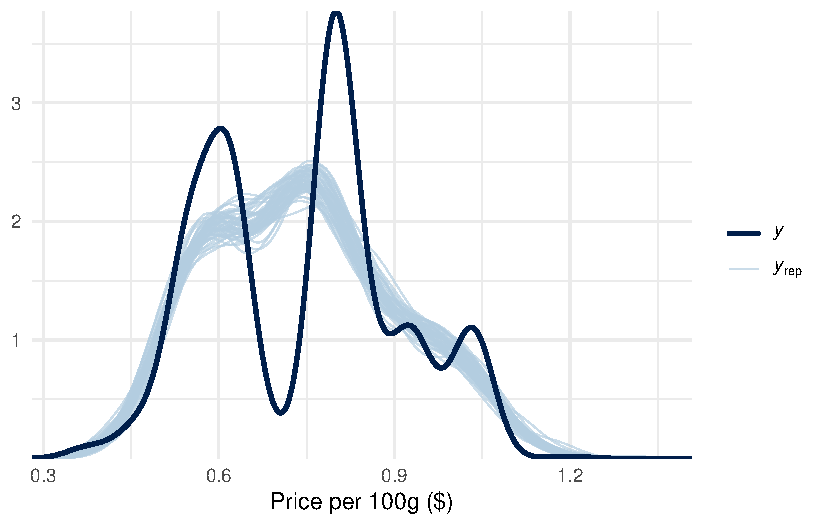
\includegraphics{paper_files/figure-pdf/fig-post-pred-1.pdf}

}

\caption{\label{fig-post-pred}Posterior predictive checks for the price
model}

\end{figure}%

\begin{figure}[H]

\centering{

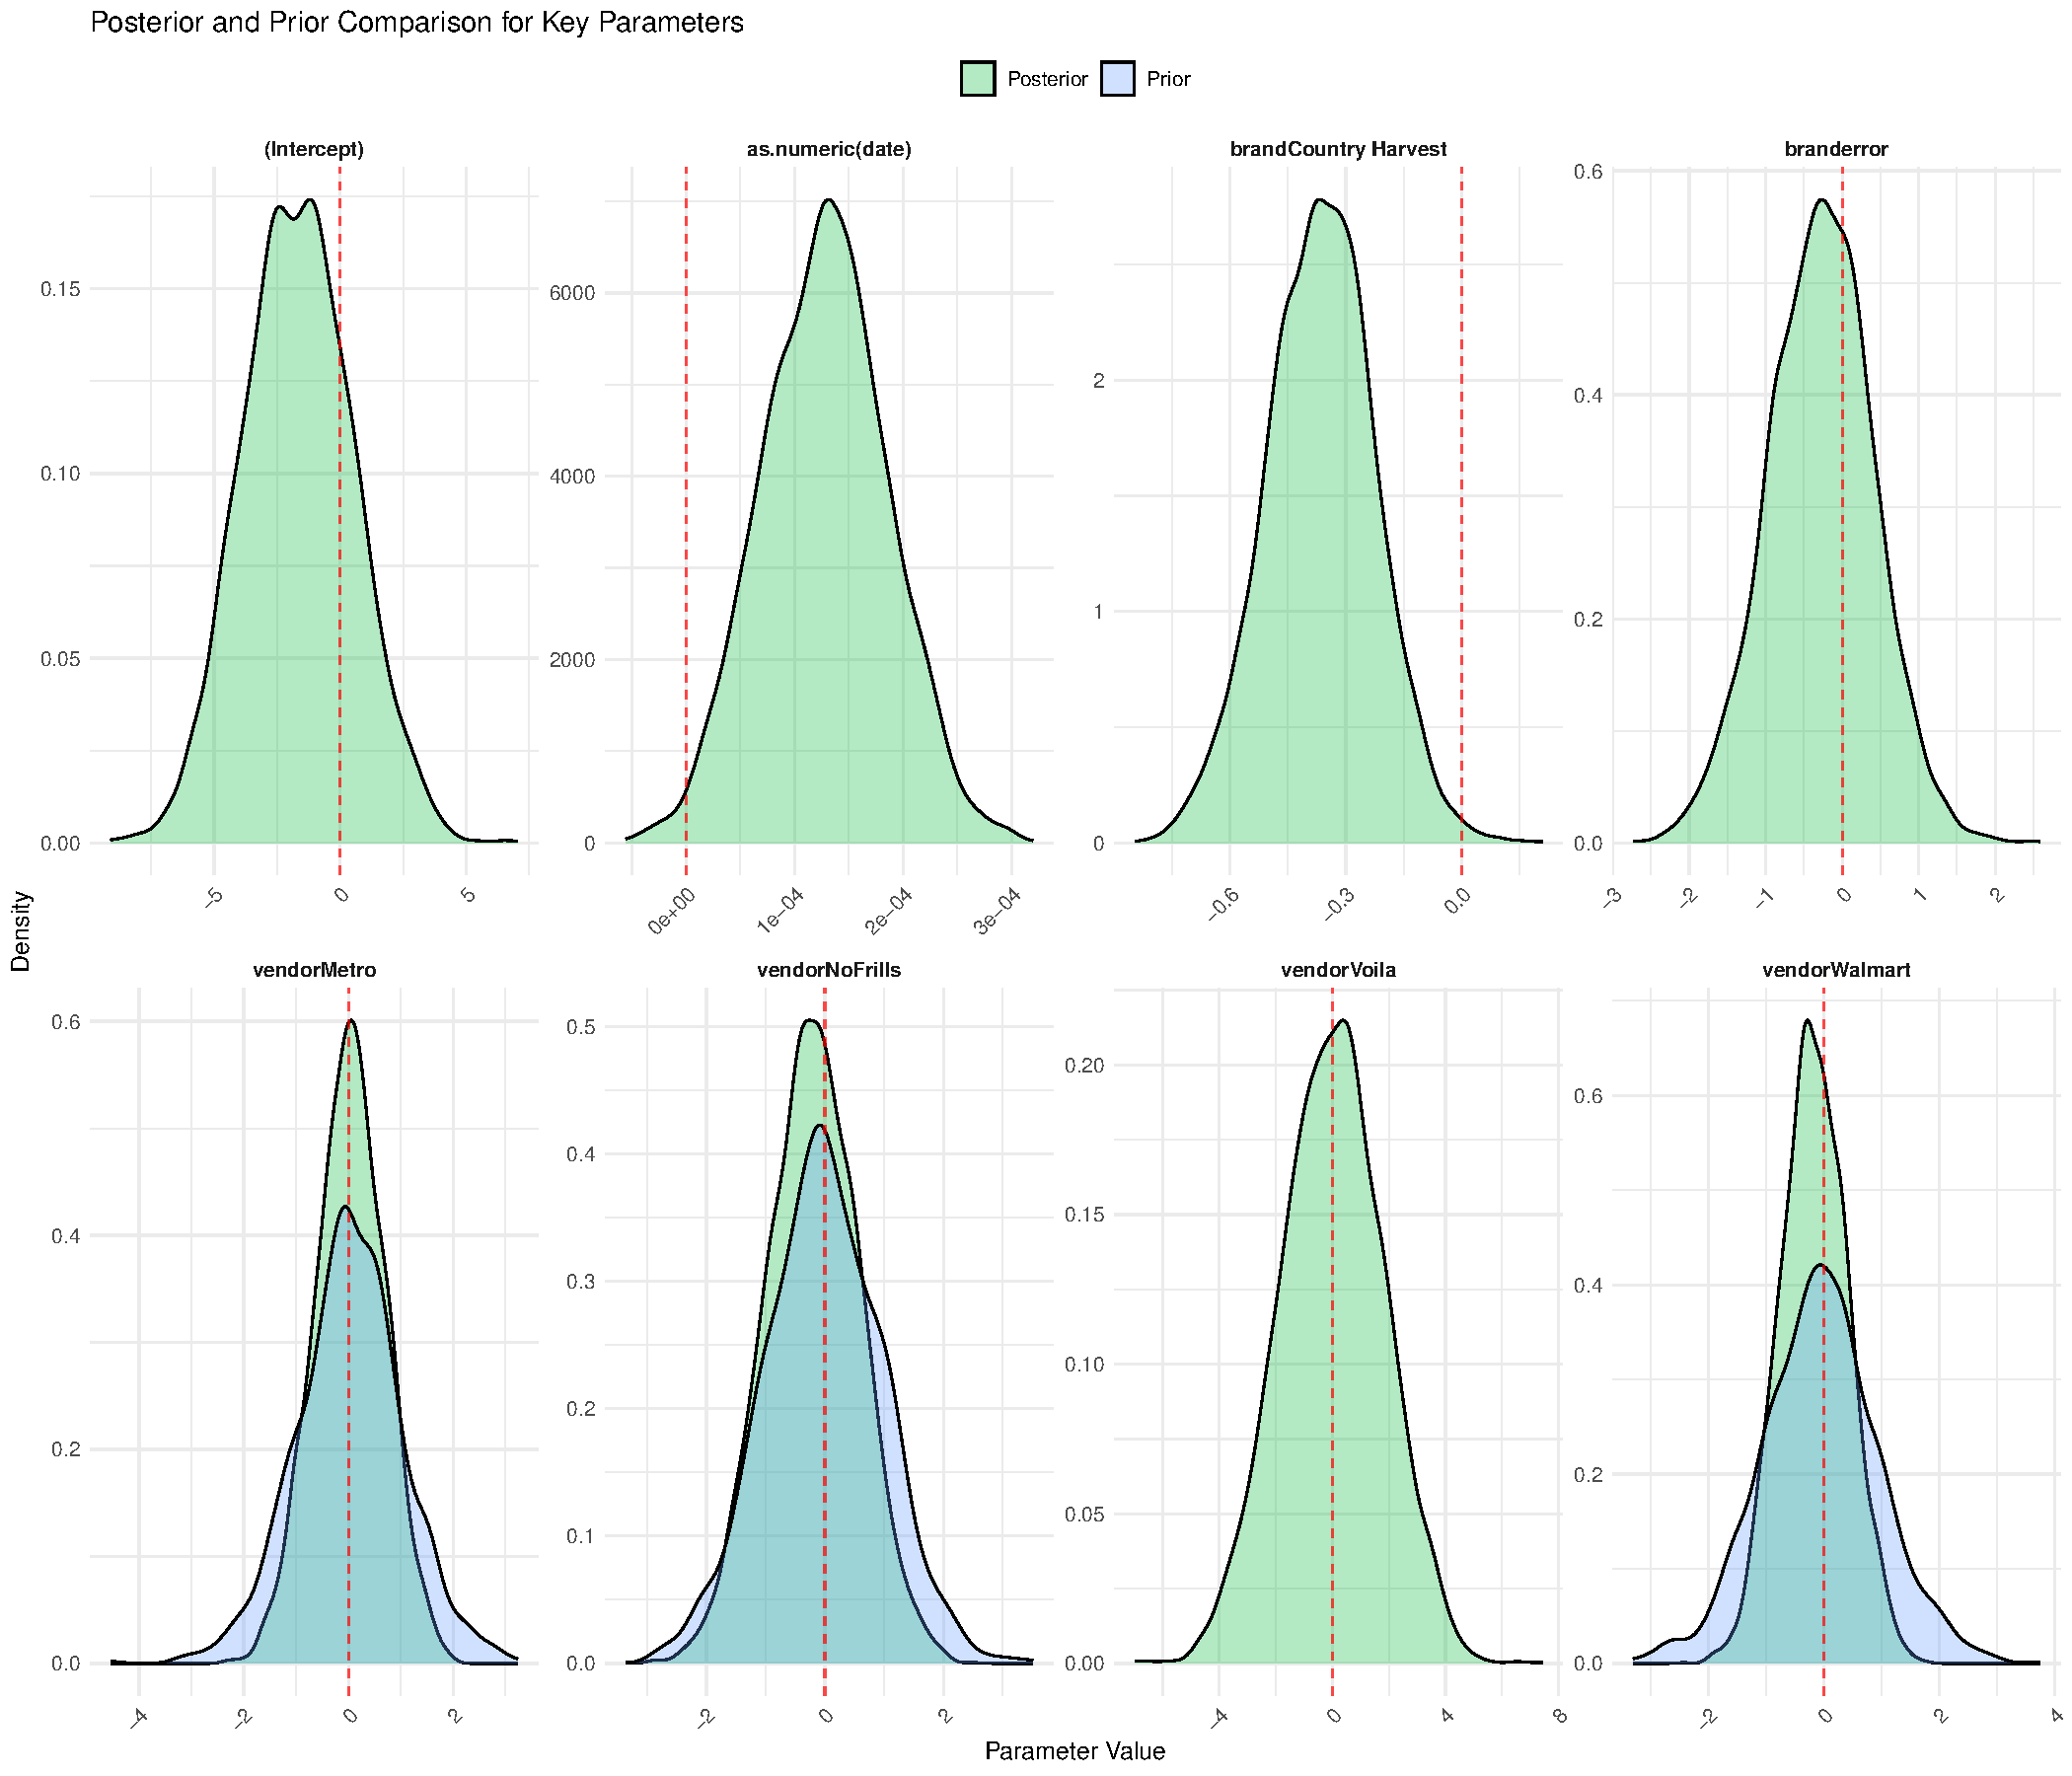
\includegraphics{paper_files/figure-pdf/fig-post-prior-1.pdf}

}

\caption{\label{fig-post-prior}Posterior and prior comparison for key
parameters}

\end{figure}%

\subsection{Diagnostics}\label{diagnostics}

\begin{figure}[H]

\centering{

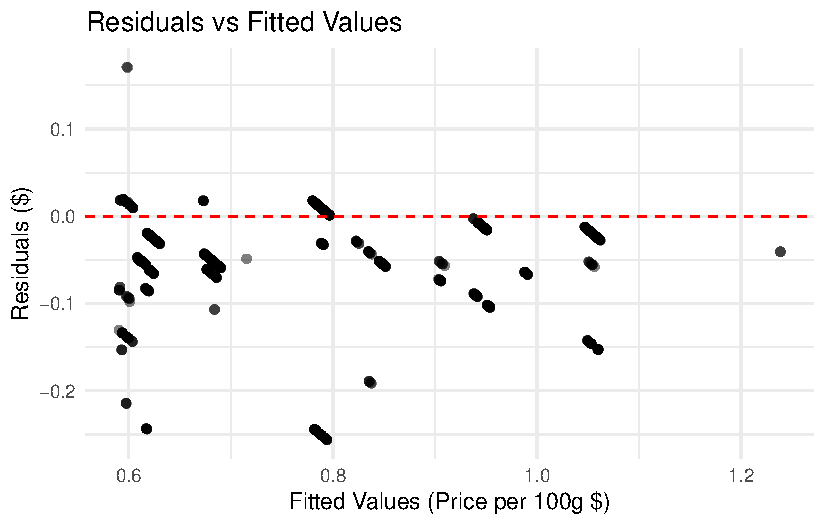
\includegraphics{paper_files/figure-pdf/fig-residuals-1.pdf}

}

\caption{\label{fig-residuals}Residual analysis plot}

\end{figure}%

\subsection{MCMC Convergence
Diagnostics}\label{mcmc-convergence-diagnostics}

\begin{figure}[H]

\centering{

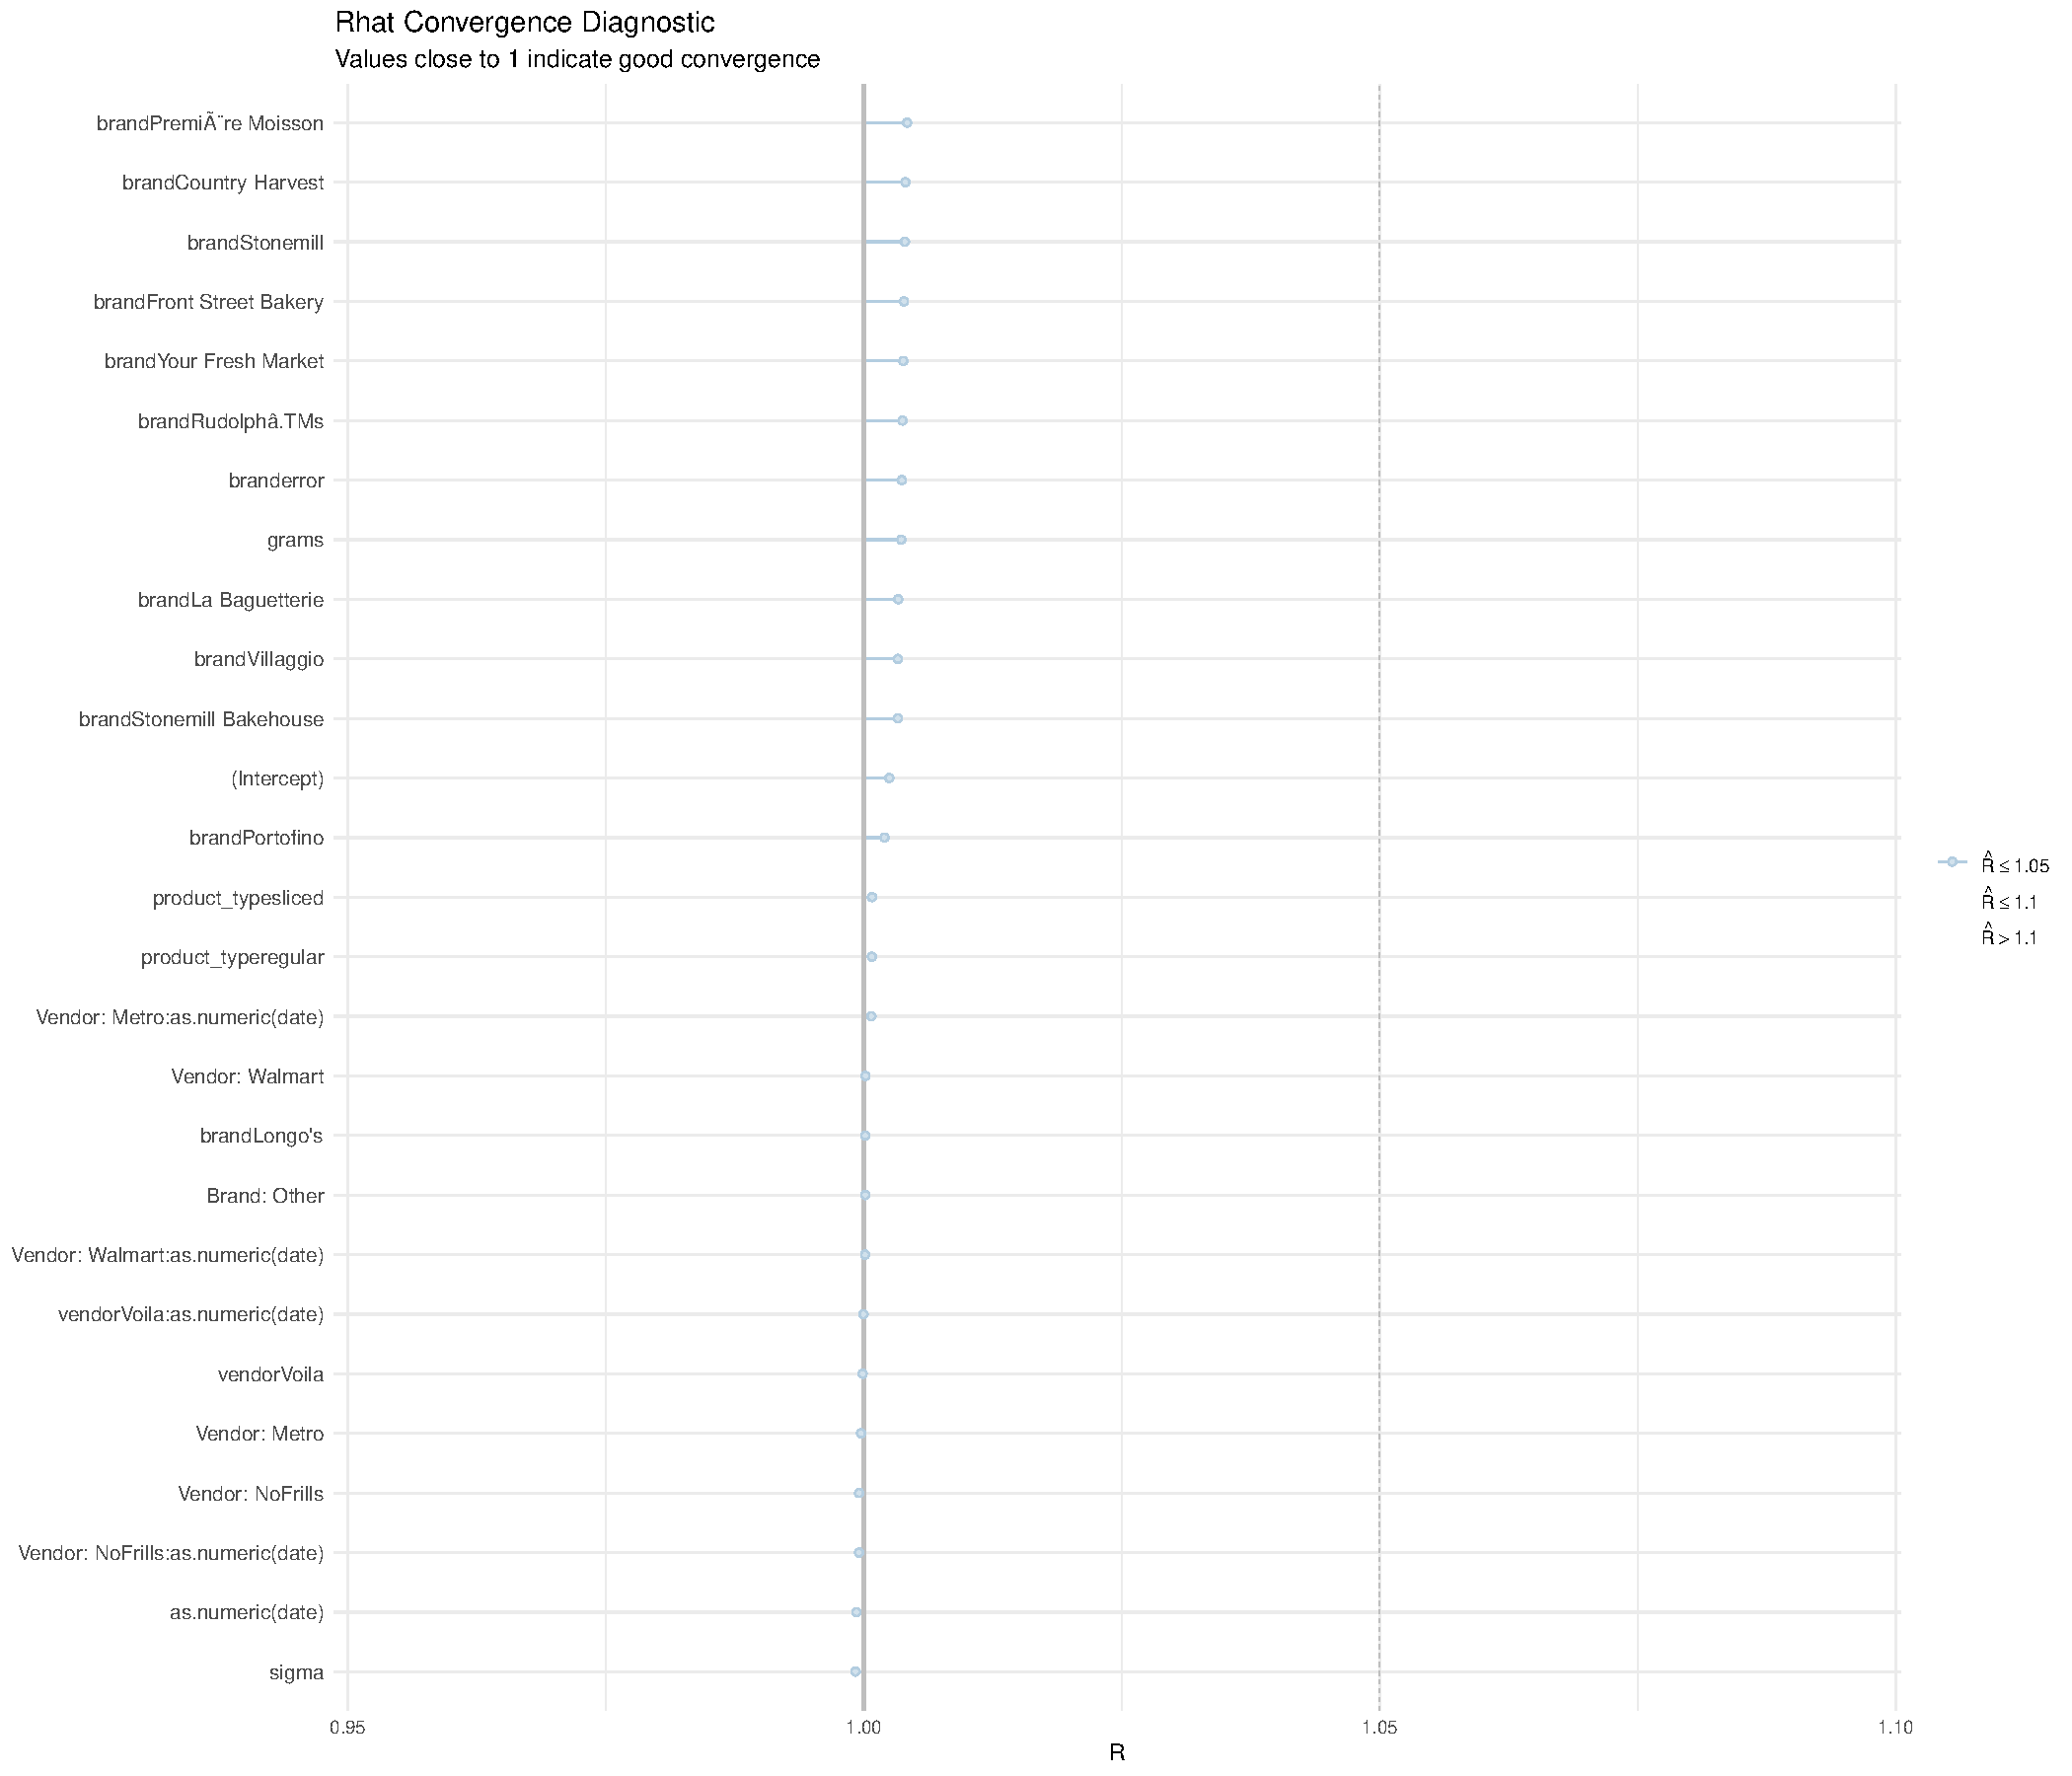
\includegraphics{paper_files/figure-pdf/fig-mcmc-convergence-1.pdf}

}

\caption{\label{fig-mcmc-convergence}Rhat Convergence Diagnostic}

\end{figure}%

\begin{figure}[H]

\centering{

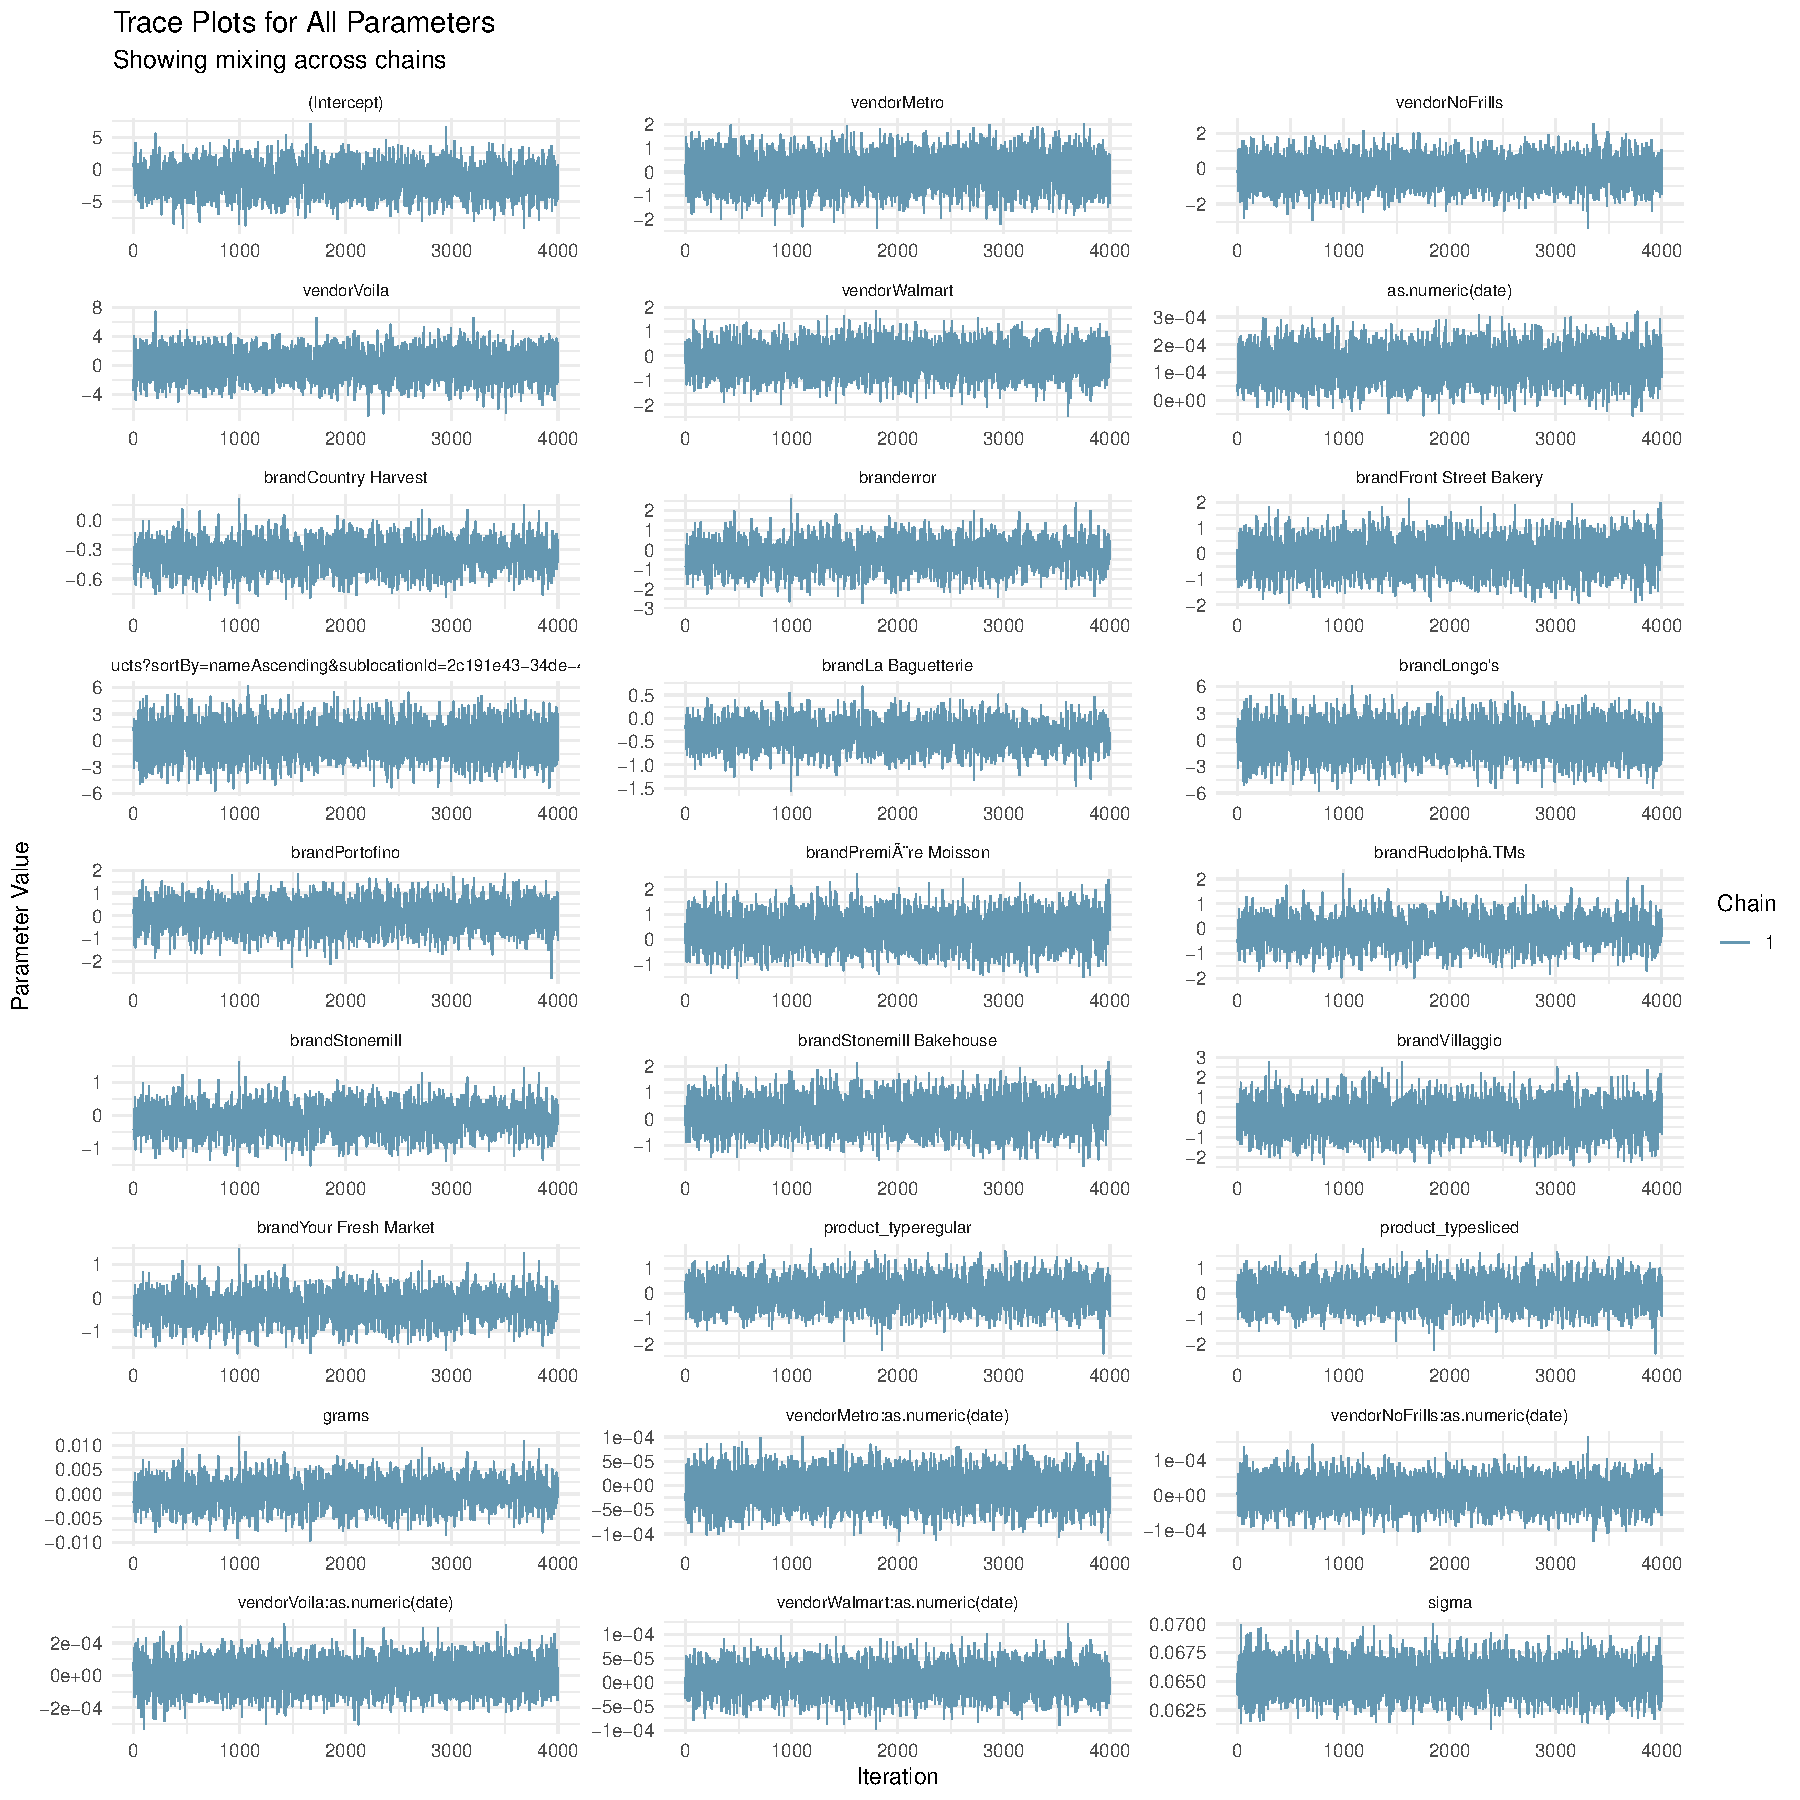
\includegraphics{paper_files/figure-pdf/fig-trace-1.pdf}

}

\caption{\label{fig-trace}Trace Plots for Key Parameters}

\end{figure}%

\section{Robustness Checks}\label{robustness-checks}

\subsection{Alternative Model
Specifications}\label{alternative-model-specifications}

Table~\ref{tbl-model-compare} present the comparison of different models
for increasing complexity

\begin{table}[H]

\caption{\label{tbl-model-compare}Comparison of model specifications
with increasing complexity}

\centering{

[H]
\centering\begingroup\fontsize{9}{11}\selectfont

\resizebox{\ifdim\width>\linewidth\linewidth\else\width\fi}{!}{
\begin{threeparttable}
\begin{tabular}{>{\raggedright\arraybackslash}p{0.8cm}>{\raggedright\arraybackslash}p{5cm}>{\centering\arraybackslash}p{1cm}>{\centering\arraybackslash}p{1cm}>{\centering\arraybackslash}p{0.8cm}}
\toprule
\multicolumn{2}{c}{ } & \multicolumn{2}{c}{Model Fit} & \multicolumn{1}{c}{ } \\
\cmidrule(l{3pt}r{3pt}){3-4}
Model & Included Variables & R² & RMSE & N\\
\midrule
Basic & Vendor + Brand & 0.720 & 0.089 & 18\\
Medium & Vendor + Brand + Product Type & 0.780 & 0.075 & 20\\
Full & Vendor × Time + Brand + Product Type + Package Size & 0.841 & 0.065 & 23\\
\bottomrule
\end{tabular}
\begin{tablenotes}[para]
\small
\item \textit{Note: } 
\item RMSE reported in dollars per 100g.
\end{tablenotes}
\end{threeparttable}}
\endgroup{}

}

\end{table}%

It shows that the Model Fit of the most complex model are better than
other models, validating our choice for this case.

\subsection{Observational Data
Considerations}\label{observational-data-considerations}

\begin{enumerate}
\def\labelenumi{\arabic{enumi}.}
\tightlist
\item
  Selection Effects:
\end{enumerate}

\begin{itemize}
\item
  Analysis of vendor availability
\item
  Product availability patterns
\item
  Price recording consistency
\end{itemize}

\begin{enumerate}
\def\labelenumi{\arabic{enumi}.}
\setcounter{enumi}{1}
\tightlist
\item
  Measurement Validation:
\end{enumerate}

\begin{itemize}
\item
  Cross-validation with multiple sources
\item
  Standard error estimation
\item
  Systematic bias assessment
\end{itemize}

\begin{enumerate}
\def\labelenumi{\arabic{enumi}.}
\setcounter{enumi}{2}
\tightlist
\item
  Sample Size Analysis:
\end{enumerate}

\begin{longtable}[t]{lrr}

\caption{\label{tbl-sample-size}Sample size adequacy analysis}

\tabularnewline

\toprule
vendor & n & power\\
\midrule
Loblaws & 76 & 1.000\\
Metro & 537 & 1.000\\
NoFrills & 178 & 1.000\\
Voila & 43 & 0.999\\
Walmart & 397 & 1.000\\
\bottomrule

\end{longtable}

\newpage

\section*{References}\label{references}
\addcontentsline{toc}{section}{References}

\phantomsection\label{refs}
\begin{CSLReferences}{1}{0}
\bibitem[\citeproctext]{ref-akerlof_2015_phishing}
Akerlof, George A, and Robert J Shiller. 2015. {``Phishing for
Phools.''} \emph{Princeton University Press} 134 (September): 115--54.
\url{https://doi.org/10.2307/j.ctvc777w8}.

\bibitem[\citeproctext]{ref-arelbundock_2022_bmodelsummaryb}
Arel-Bundock, Vincent. 2022. {``Modelsummary: Data and Model Summaries
in r.''} \emph{Journal of Statistical Software} 103 (January).
\url{https://doi.org/10.18637/jss.v103.i01}.

\bibitem[\citeproctext]{ref-barnett_2007_weather}
Barnett, Barry J., and Olivier Mahul. 2007. {``Weather Index Insurance
for Agriculture and Rural Areas in Lower‐income Countries.''}
\emph{American Journal of Agricultural Economics} 89 (December):
1241--47. \url{https://doi.org/10.1111/j.1467-8276.2007.01091.x}.

\bibitem[\citeproctext]{ref-basker_2007_the}
Basker, Emek. 2007. {``The Causes and Consequences of Wal-Mart's
Growth.''} \emph{Journal of Economic Perspectives} 21 (July): 177--98.
\url{https://doi.org/10.1257/jep.21.3.177}.

\bibitem[\citeproctext]{ref-dellavigna_2019_uniform}
DellaVigna, Stefano, and Matthew Gentzkow. 2019. {``Uniform Pricing in
u.s. Retail Chains.''} \emph{The Quarterly Journal of Economics} 134
(June): 2011--84. \url{https://doi.org/10.1093/qje/qjz019}.

\bibitem[\citeproctext]{ref-apachearrowdevelopers_2023_arrow}
Developers, Apache Arrow. 2023. {``Arrow r Package.''} Apache.org.
\url{https://arrow.apache.org/docs/r/}.

\bibitem[\citeproctext]{ref-dubois_2010_price}
Dubois, Pierre, and Sandra Jodar-Rosell. 2010. {``Price and Brand
Competition Between Differentiated Retailers: A Structural Econometric
Model.''} Ssrn.com. \url{https://ssrn.com/abstract=1640369}.

\bibitem[\citeproctext]{ref-ellickson_2008_supermarket}
Ellickson, Paul B., and Sanjog Misra. 2008. {``Supermarket Pricing
Strategies.''} \emph{Marketing Science} 27: 811--28.
\url{https://www.jstor.org/stable/40057128}.

\bibitem[\citeproctext]{ref-filipp_2024_project}
Filipp, Jacob. 2024. {``Project Hammer -- Jacob Filipp.''}
Jacobfilipp.com. \url{https://jacobfilipp.com/hammer/}.

\bibitem[\citeproctext]{ref-goodrich_2023_bayesian}
Goodrich, Ben, Jonah Gabry, Imad Ali, and Sam Brilleman. 2023.
{``Bayesian Applied Regression Modeling via Stan.''} mc-stan.org.
\url{https://mc-stan.org/rstanarm/}.

\bibitem[\citeproctext]{ref-hausman_2007_consumer}
Hausman, Jerry, and Ephraim Leibtag. 2007. {``Consumer Benefits from
Increased Competition in Shopping Outlets: Measuring the Effect of
Wal-Mart.''} \emph{Journal of Applied Econometrics} 22: 1157--77.
\url{https://doi.org/10.1002/jae.994}.

\bibitem[\citeproctext]{ref-kaplan_2019_relative}
Kaplan, Greg, Guido Menzio, Leena Rudanko, and Nicholas Trachter. 2019.
{``Relative Price Dispersion: Evidence and Theory.''} \emph{American
Economic Journal: Microeconomics} 11 (August): 68--124.
\url{https://doi.org/10.1257/mic.20170126}.

\bibitem[\citeproctext]{ref-nakamura_2011_price}
Nakamura, Emi, and Jón Steinsson. 2011. {``Price Setting in
Forward-Looking Customer Markets.''} \emph{Journal of Monetary
Economics} 58 (April): 220--33.
\url{https://doi.org/10.1016/j.jmoneco.2011.06.004}.

\bibitem[\citeproctext]{ref-seiler_2017_the}
Seiler, Stephan, and Song Yao. 2017. {``The Impact of Advertising Along
the Conversion Funnel.''} \emph{SSRN Electronic Journal} 15: 241--78.
\url{https://doi.org/10.2139/ssrn.2920953}.

\bibitem[\citeproctext]{ref-rcoreteam_2024_r}
Team, R Core. 2024. {``R: A Language and Environment for Statistical
Computing.''} R Foundation for Statistical Computing.
\url{https://www.r-project.org/}.

\bibitem[\citeproctext]{ref-wickham_2016_create}
Wickham, Hadley. 2016. {``Create Elegant Data Visualisations Using the
Grammar of Graphics.''} Tidyverse.org.
\url{https://ggplot2.tidyverse.org/}.

\bibitem[\citeproctext]{ref-wickham_2019_welcome}
Wickham, Hadley, Mara Averick, Jennifer Bryan, Winston Chang, Lucy
McGowan, Romain François, Garrett Grolemund, et al. 2019. {``Welcome to
the Tidyverse.''} \emph{Journal of Open Source Software} 4 (November):
1686. \url{https://doi.org/10.21105/joss.01686}.

\end{CSLReferences}




\end{document}
